% -----------------------------------------------
% Template for SMC 2020
% adapted from previous SMC paper templates
% -----------------------------------------------

\documentclass[dvipsnames, pdftex]{article}
\usepackage{smc2020}
\usepackage{times}
\usepackage{ifpdf}
\usepackage[english]{babel}
\usepackage{cite}
\usepackage{amsmath}
\usepackage{textcomp}

\usepackage{xcolor}
\def\SWcomment[#1]{\textcolor{Red}{#1}}
\def\RPcomment[#1]{\textcolor{Blue}{#1}}
\def\SScomment[#1]{\textcolor{OliveGreen}{#1}}

%%%%%%%%%%%%%%%%%%%%%%%% Some useful packages %%%%%%%%%%%%%%%%%%%%%%%%%%%%%%%
%%%%%%%%%%%%%%%%%%%%%%%% See related documentation %%%%%%%%%%%%%%%%%%%%%%%%%%
%\usepackage{amsmath} % popular packages from Am. Math. Soc. Please use the 
%\usepackage{amssymb} % related math environments (split, subequation, cases,
%\usepackage{amsfonts}% multline, etc.)
%\usepackage{bm}      % Bold Math package, defines the command \bf{}
%\usepackage{paralist}% extended list environments
%%subfig.sty is the modern replacement for subfigure.sty. However, subfig.sty 
%%requires and automatically loads caption.sty which overrides class handling 
%%of captions. To prevent this problem, preload caption.sty with caption=false 
%\usepackage[caption=false]{caption}
%\usepackage[font=footnotesize]{subfig}


%user defined variables
\def\papertitle{Resurrecting the Tromba Marina: a Bowed Virtual Reality Instrument using Haptic Feedback and Accurate Physical Modelling}

\def\firstauthor{Silvin Willemsen}
\def\secondauthor{Razvan Paisa}
\def\thirdauthor{Stefania Serafin}

% adds the automatic
% Saves a lot of output space in PDF... after conversion with the distiller
% Delete if you cannot get PS fonts working on your system.

% pdf-tex settings: detect automatically if run by latex or pdflatex
\newif\ifpdf
\ifx\pdfoutput\relax
\else
   \ifcase\pdfoutput
      \pdffalse
   \else
      \pdftrue
\fi

\ifpdf % compiling with pdflatex
  \usepackage[pdftex,
    pdftitle={\papertitle},
    pdfauthor={\firstauthor, \secondauthor, \thirdauthor},
    bookmarksnumbered, % use section numbers with bookmarks
    pdfstartview=XYZ % start with zoom=100% instead of full screen; 
                     % especially useful if working with a big screen :-)
   ]{hyperref}
  %\pdfcompresslevel=9

  \usepackage[pdftex]{graphicx}
  % declare the path(s) where your graphic files are and their extensions so 
  %you won't have to specify these with every instance of \includegraphics
  \graphicspath{{./figures/}}
  \DeclareGraphicsExtensions{.pdf,.jpeg,.png}

  \usepackage[figure,table]{hypcap}

\else % compiling with latex
  \usepackage[dvips,
    bookmarksnumbered, % use section numbers with bookmarks
    pdfstartview=XYZ % start with zoom=100% instead of full screen
  ]{hyperref}  % hyperrefs are active in the pdf file after conversion

  \usepackage[dvips]{epsfig,graphicx}
  % declare the path(s) where your graphic files are and their extensions so 
  %you won't have to specify these with every instance of \includegraphics
  \graphicspath{{./figures/}}
  \DeclareGraphicsExtensions{.eps}

  \usepackage[figure,table]{hypcap}
\fi

%setup the hyperref package - make the links black without a surrounding frame
\hypersetup{
    colorlinks,%
    citecolor=black,%
    filecolor=black,%
    linkcolor=black,%
    urlcolor=black
}


% Title.
% ------
\title{\papertitle}

% Authors
% Please note that submissions are NOT anonymous, therefore 
% authors' names have to be VISIBLE in your manuscript. 
%
% Single address
% To use with only one author or several with the same address
% ---------------
\oneauthor
   {\firstauthor, \secondauthor\ and \thirdauthor} {Multisensory Experience Lab, CREATE\\
  Aalborg University Copenhagen\\ %
    {\tt \href{mailto:sil@create.aau.dk}{\{sil, rpa, sts\}@create.aau.dk}}}

%Two addresses
%--------------
% \twoauthors
%   {\firstauthor} {Affiliation1 \\ %
%     {\tt \href{mailto:author1@smcnetwork.org}{author1@smcnetwork.org}}}
%   {\secondauthor} {Affiliation2 \\ %
%     {\tt \href{mailto:author2@smcnetwork.org}{author2@smcnetwork.org}}}

% Three addresses
% --------------
%  \threeauthors
%   {\firstauthor} {Affiliation1 \\ %
%      {\tt \href{mailto:author1@smcnetwork.org}{author1@smcnetwork.org}}}
%   {\secondauthor} {Affiliation2 \\ %
%      {\tt \href{mailto:author2@smcnetwork.org}{author2@smcnetwork.org}}}
%   {\thirdauthor} { Affiliation3 \\ %
%      {\tt \href{mailto:author3@smcnetwork.org}{author3@smcnetwork.org}}}


% ***************************************** the document starts here ***************
\begin{document}
%
\capstartfalse
\maketitle
\capstarttrue
%
\begin{abstract}
In this paper we propose a multisensory simulation of a tromba marina - a bowed string instrument in virtual reality. The auditory feedback is generated by an accurate physical model, the haptic feedback is provided by the PHANTOM Omni, and the visual feedback is rendered through an Oculus Rift CV1 head-mounted display (HMD). Moreover, we present a user study exploring the experience of interacting with a virtual bowed string instrument, as well as evaluating the playability of the system. The study comprises of both qualitative (observations, think aloud and interviews) and quantitative (survey) data collection methods. The results indicate that the implementation was successful, offering participants realistic feedback, as well as a satisfactory multisensory experience, allowing them to use the system as a musical instrument.
\end{abstract}

\section{Introduction}\label{sec:introduction}
The tromba marina is a bowed monochord from medieval Europe \cite{encyclopaedia2020}. The string rests on a loose bridge that rattles against the body. This rattling mechanism creates a sound with brass- or trumpet-like qualities. Unlike other bowed string instruments, different frequencies are created by slightly damping the string with a finger of the non-bowing hand as opposed to pressing the string fully against the neck. This interaction at different locations along the string triggers the different harmonics of the open string. Furthermore, the tromba marina is bowed closer to the nut, and the finger determining the frequency is closer to the bridge (below the bow).
As the tromba marina is a rare instrument which can be merely found in museums, very few have the opportunity to play it and discover its interesting timbral possibilities. 
We wish to recreate the feeling of playing this instrument by using physics based  multisensory simulations \cite{pai2005multisensory}.

In the context of musical applications, physics based multisensory simulations have shown some interest in the sound and music computing community. 
As stated in 
\cite{danieau2012enhancing}, the combination of haptics and audio visual content has its own specific challenges worth investigating.
Sile O'Modhrain is one of the pioneers that noticed the tight connection between auditory and haptic feedback and investigated how haptic feedback can improve the playability of virtual instruments \cite{o2001playing}.
At the same time, Charles Nichols developed the vBow, a haptic human computer interface for bowing \cite{nichols2002vbow}.
Researchers from ACROE in Grenoble have developed for several years multisensory instruments based on the mass-spring-system paradigm, with custom-made bowing interfaces \cite{florens1990modeles,luciani2005action}.
Such multisensory simulations have recently been made open source \cite{villeneuve2019mass}.
Haptic feedback has also been combined with digital waveguide models for simulating bowed string interactions \cite{sinclair2009audio}.

Simulating the vibrations' feeling of a string instrument is particularly important since it has been shown how vibration's level can be strongly perceived \cite{askenfelt1992vibration}. 
We use democratized VR technologies controlled by a commercial device called the PHANTOM Omni (or simply Omni) by SenseAble Technologies (now 3D Systems) \cite{phantom}.
The Omni is a six-degrees-of-freedom system providing the tracking and haptic feedback in our application.
Using the same device, Avanzini and Crosato tested the influence of haptic and auditory cues on perception of material stiffness   \cite{avanzini2006}.
Auditory stimuli were obtained using a physically-based audio model of impact, in which the colliding objects are described as modal resonators that interact through a non-linear impact force \cite{avanzini2004physical}.
Auditory stiffness was varied while haptic stiffness was kept constant. Results show a significant interaction between auditory stiffness and haptic stiffness, the first affecting the perception of the second. Passalenti et. al's also used the Omni to simulate the act of plucking a virtual guitar string \cite{passalenti2019a, passalenti2019b, Fontana2020}.

%We want to emphasize that the visuals are only used for guiding the user, as we are most interested in the haptic feedback and audio.

The goal of this project is to explore the experience of interacting with virtual bowed instrument by using physics based simulations and haptic feedback, together with a visual virtual reality (VR) experience. This effectively makes the implementation a virtual reality musical instrument (VRMI) \cite{Serafin2016}. The tromba marina is used solely as inspiration because it affords itself to being a solid starting point by having only one string. Besides that, the rarity of the instrument ensures that the participants do not have prior experience playing a tromba marina, nullifying possible comparisons between a real instrument and the virtual one. At no point the system was evaluated as an alternative to the real tromba marina. The system (and its evaluation) is targeted towards musicians in order to avoid discouragement frequently encountered when non-musicians interact with musical instruments. It is assumed that musicians acknowledge that mastering any instrument require extended study, therefore it is expected that they will not evaluate this system exclusively based on its difficulty to play.

We start by describing the implementation of the system, both from the hardware and software perspective in Section \ref{sec:implementation}, followed by presenting a study that evaluates the setup in Section \ref{sec:eval}. Section \ref{sec:results} shows the results of the evaluation and Section \ref{sec:discussion} discusses these. Finally, concluding remarks appear in \ref{sec:conclusion}.

\section{Implementation}\label{sec:implementation}
The virtual tromba marina consists of three main components: auditory, visual and haptic feedback, all of which will be elaborated on in this section. Then controls and mapping and the final setup of the system will be presented. A video showing the implementation can be found in \cite{Trombavideo2020}.

\subsection{Auditory feedback}
The audio is generated by a physical model of the tromba marina presented in a companion paper \cite{Willemsen2020}. Some parameters of the model are exposed and can be controlled by the user. These are the velocity, force and position of the bow and the position of the finger inducing the harmonics. The algorithm will not be discussed in detail here, but the mapping to the various parameters of the model will be described in Section \ref{sec:controls}.

\subsection{Visual feedback}
The application was built using the cross-platform game engine Unity3D \cite{unity} which can be used to build VR applications. Even though the visual feedback is not the focus of the implementation and eventual evaluation, it was used to guide the users' movements and give them a sense of where the virtual instrument was located. For the implementation an Oculus Rift CV1 setup was used \cite{Oculus2020}. Figure \ref{fig:vrView} shows a screenshot of the view from the head-mounted display (HMD), depicting the virtual instrument, the bow and the damping finger indicator. A 3D model of the tromba marina was made inspired by a real-life instrument (presented in \cite{Baldwin2016}) available to the authors. The overall environment resembled a medieval room, providing context to tromba marina's historical nature.

\begin{figure}[ht]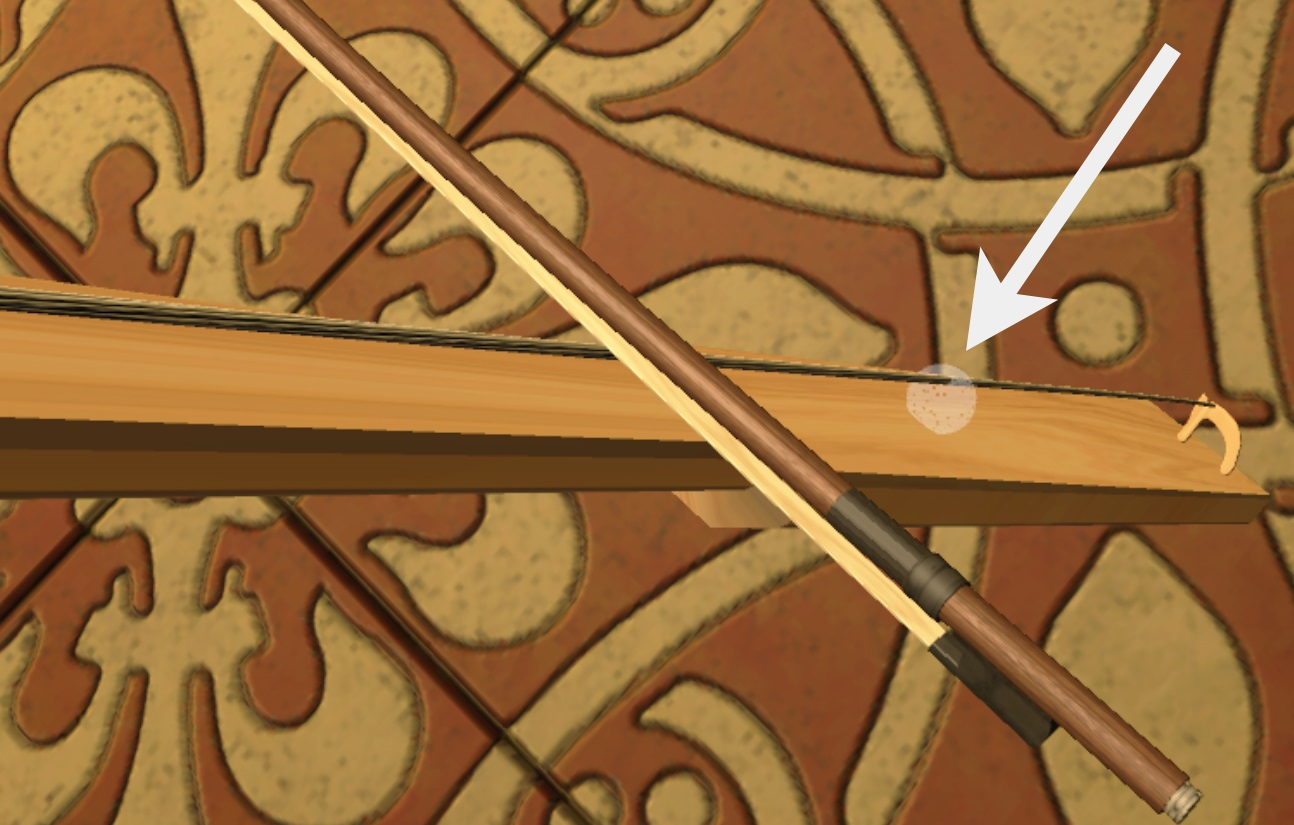
\includegraphics[width=1.0\columnwidth]{SMC 2020 paper template LaTeX/figures/vrView.jpg}
\centering
  \caption{The view from the head-mounted display (HMD). The damping finger is highlighted and shown as a transparent white sphere. \label{fig:vrView}}
\end{figure}

\subsection{Haptic feedback}
The PHANTOM Omni (or simply Omni) is a six-degrees-of-freedom tracking and haptic system developed by SensAble Technologies (see Figure \ref{fig:omni}). The device has a pen-shaped arm that a user interacts with.  

\begin{figure}[t]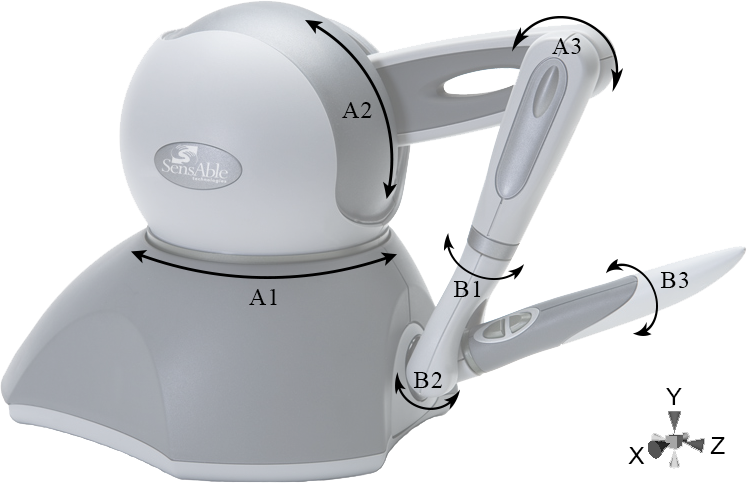
\includegraphics[width=1.0\columnwidth]{figures/omniSchematic.png}
\centering
  \caption{The PHANTOM Omni has six axes of rotation, three of which provide force feedback (A1-3), and three only tracking position (B1-3). Together, these axes provide six degrees of freedom: x, y and z positions of B2 and rotations of the pen. \label{fig:omni}}
\end{figure}

The raw data provided by the Omni is 1) the absolute position of pivot point B2 (three degrees of freedom), 2) the rotation (three degrees of freedom), and 3) the pressure (touching depth).

The axes are labelled as follows in relation to the virtual tromba marina (also see global coordinate system in Figure \ref{fig:localGlobal}): x-axis (width): horizontally across the soundboard (the common interaction direction), y-axis (height): floor to ceiling, and z-axis (depth): perpendicular to the soundboard.

The end of the bow -- where a user normally holds it -- has been placed at pivot point B2. The fact that pivot points B1-3 do not provide force feedback gives rise to an issue in our application. If the virtual
position of pivot point B2 is not the current point of interaction, in the extreme case when the user is bowing using the end of the bow, a force has to be applied as to still provide haptic feedback. To solve this issue, we created a separate game object with which the bow (pivot point B2 to be exact) will interact with in the virtual world Figure \ref{fig:localGlobal}. This `(hidden) collision block' lives in a local coordinate system and its x and y-position exactly follow that of the Omni-pen. The y-rotation will change the rotation of the local coordinate system and uses the virtual string as the center point. If, for any reason, the bow ends up behind the string, the collision block will be offset to the left along the (local) x-axis so that no collision occurs when trying to return the bow to the normal playing area. 

\begin{figure}[ht]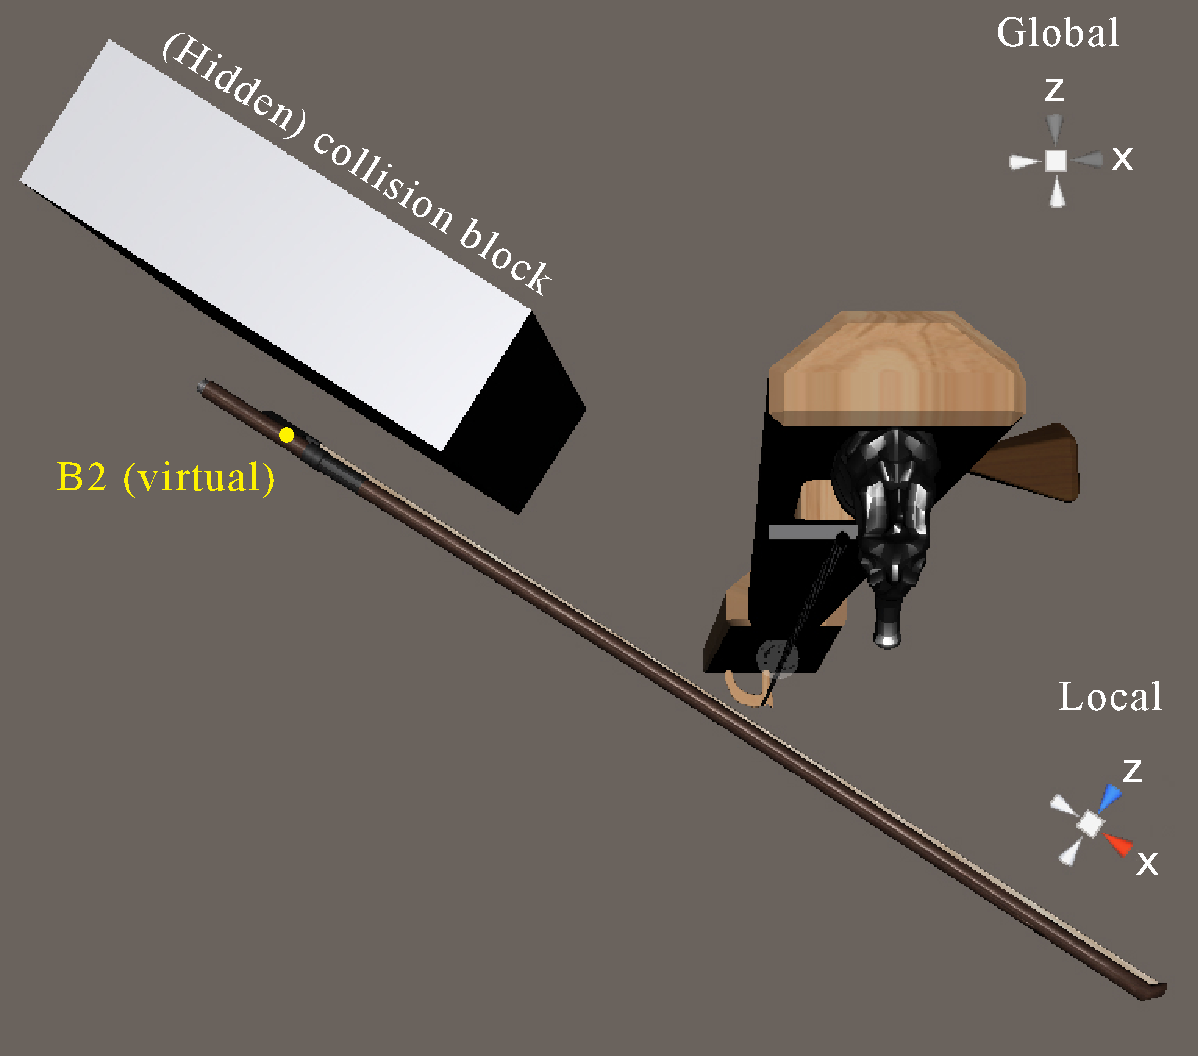
\includegraphics[width=1.0\columnwidth]{SMC 2020 paper template LaTeX/figures/globalLocal.pdf}
\centering
  \caption{Top-down view of the global and local coordinate system (x-z--plane). The rotation of the local coordinate system around the (global) y-axis is determined by the y-rotation of the bow. The (normally hidden) collision block lives in the local coordinate system. Its (local) x and y-position follows the (local) x and y-position of B2. \label{fig:localGlobal}}
\end{figure}

The API of the Omni provides a list of pseudophysical parameters on which the haptic feedback greatly depends. Through emperical testing, the pseudophysical parameters in Table \ref{tab:pseudoParams} have been found. For more information, please refer to \cite{OmniAPI2018}. 
\begin{table}[h]
    \centering
    \begin{tabular}{|c|c|}
    \hline
        Parameter & Value \\\hline
        Stiffness & $0.003$ \\
        Damping & $0.0071$ \\
        Static Friction & 0 \\
        Dynamic Friction & 0.109 \\ 
        Pop-through & 0\\\hline
    \end{tabular}
    \caption{Pseudophysical parameters chosen for the haptics.}
    \label{tab:pseudoParams}
\end{table}

Throughout implementation, it was considered to actuate the Haptic Omni's pen with vibrotatctile stimuli, in order to replicate the stick-slip interaction encountered in a real bowing scenario. This was deemed unnecessary, as the Omni's internal gearing systems provide a similar, though uncorrelated, haptic feedback, which satisfied the authors.  

\subsection{Controls and Mapping}\label{sec:controls}
As most people are right-handed, it was chosen to also have the bow in the right hand in the application. The (now-local) x-velocity of the Omni is mapped to the bow velocity, pressure to bow force and y-position (including rotation around the local z-axis) to bow position. The left hand is used to control the pitch by changing the position of the damping finger along the string. This position is defined as  
\begin{equation}\label{eq:node}
    x_\text{f} = L\cdot n^{-1},
\end{equation}
where $L$ is the length of the string and $n \in [2,8]$. If $n$ is an integer, it is the number of the harmonic we want to induce. The lowest harmonic has been set at half the string length $L/2$, meaning that the string is never completely open. The highest harmonic (8 in this case) has been chosen to be the one that can still be (comfortably) reached. The location of the damping finger $x_\text{f}$ is controlled using the `X' and `Y' buttons and the joystick on the left Oculus controller. % (see Figure \ref{fig:oculusController}). 
The buttons are used for ``discrete harmonic" control of the damping finger, i.e. integer values of $n$ in Equation \eqref{eq:node}, where `Y' increases $n$ and `X' decreases it. The joystick allows for fine pitch control, i.e., decimal values of $n$, and moves the damping finger up and down the string. The latter could potentially create pitch glides in the output sound of the application, but make it harder to `hit' a perfect harmonic according to Equation \eqref{eq:node}. It is worth mentioning that the effect of the joystick's movement on position was scaled down to 0.3, based on empirical tests.  If a button is pressed while the current finger position is between two discrete points, the position will move to the next or previous discrete position, depending on the button pressed.
%As the position of the first node along the string is at \begin{equation}\label{eq:node}
%     x_\text{node} = L\cdot n^{-1},
% \end{equation}
% where $L$ is the length of the string and $n \in [2,8]$ is the harmonic number, we want the damping finger to be set to these positions to induce these harmonics. The lowest harmonic has been set at half the string length $L/2$, meaning that the string is never completely open. The highest harmonic has been chosen to be the one that can still be (comfortably) played. The location of the damping finger ($x_\text{f}$) is controlled using the `X' and `Y' buttons and the joystick on the left Oculus controller (see Figure \ref{fig:oculusController}). The buttons are for discrete control of the damping finger, where `Y' increases $n$ in Equation \eqref{eq:node} and `X' decreases it. The joystick allows for fine pitch control  and moves the damping finger up and down the string. The latter could potentially create pitch glides in the output sound of the application, but make it harder to `hit' a perfect harmonic according to Equation \eqref{eq:node}. If a button is pressed while the current finger position is between two discrete points, the position will move to the next or previous discrete position, depending on the button pressed.

% \begin{figure}[ht]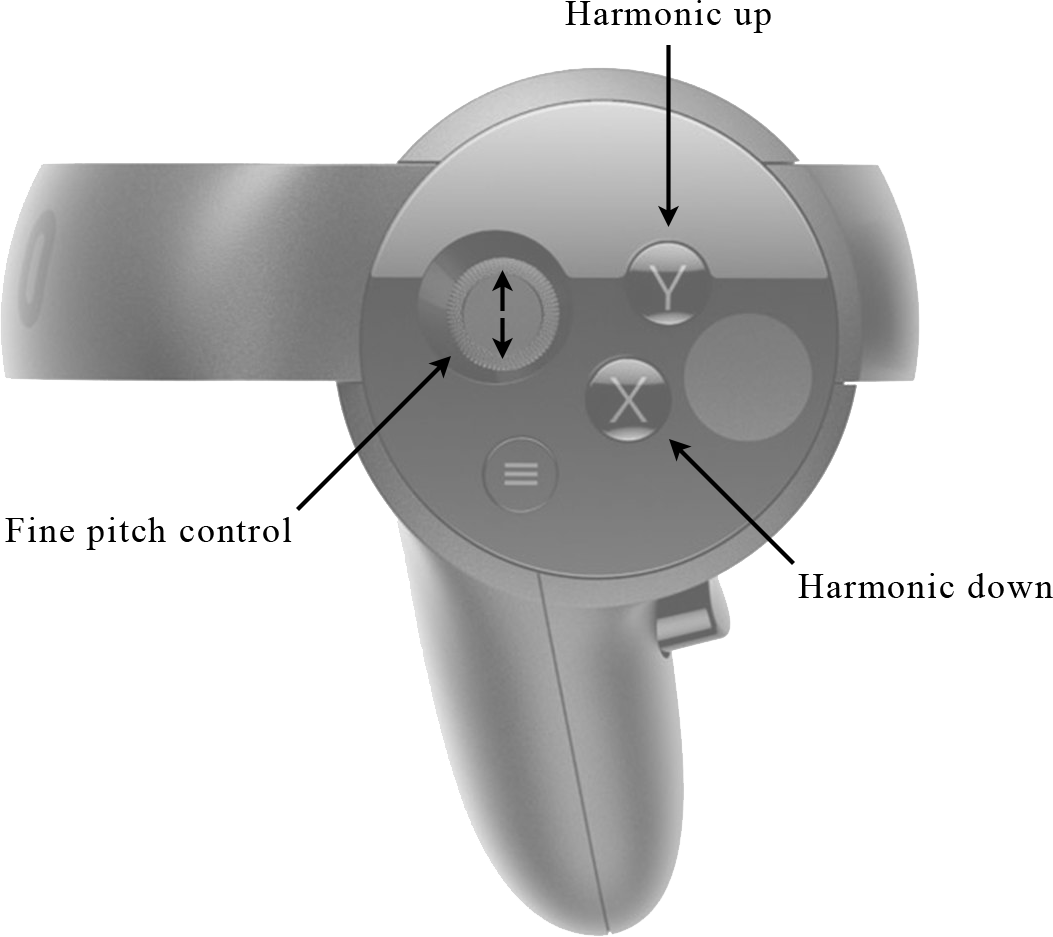
\includegraphics[width=1.0\columnwidth]{SMC 2020 paper template LaTeX/figures/controller.png}
% \centering
%   \caption{The left Oculus Touch controller. The controls for changing the pitch are highlighted. \label{fig:oculusController}}
% \end{figure}
\subsection{Physical setup}\label{subsec:physicalSetup}
The physical setup is shown in Figure \ref{fig:physicalSetup}. The Omni is mounted on a stand at \texttildelow125 cm to match the approximate bowing height of the real instrument. As can be seen in Figure \ref{fig:physicalSetup}, the right Oculus Touch controller is mounted right underneath the Omni. This is used to align the physical setup with the virtual tromba marina, both in the x-z--plane but also the height of the bow in the application. After the scene is initialised the controller is used for a tilting interaction so that the instrument can rest on the user's body, as is done with the real instrument. The aforementioned alignment came with a drawback. As the center of the x-axis range of the Omni was aligned with the tromba marina and B2 was aligned with one end of the bow, only half of the range of the Omni could be used for bowing.

% \begin{figure}[ht]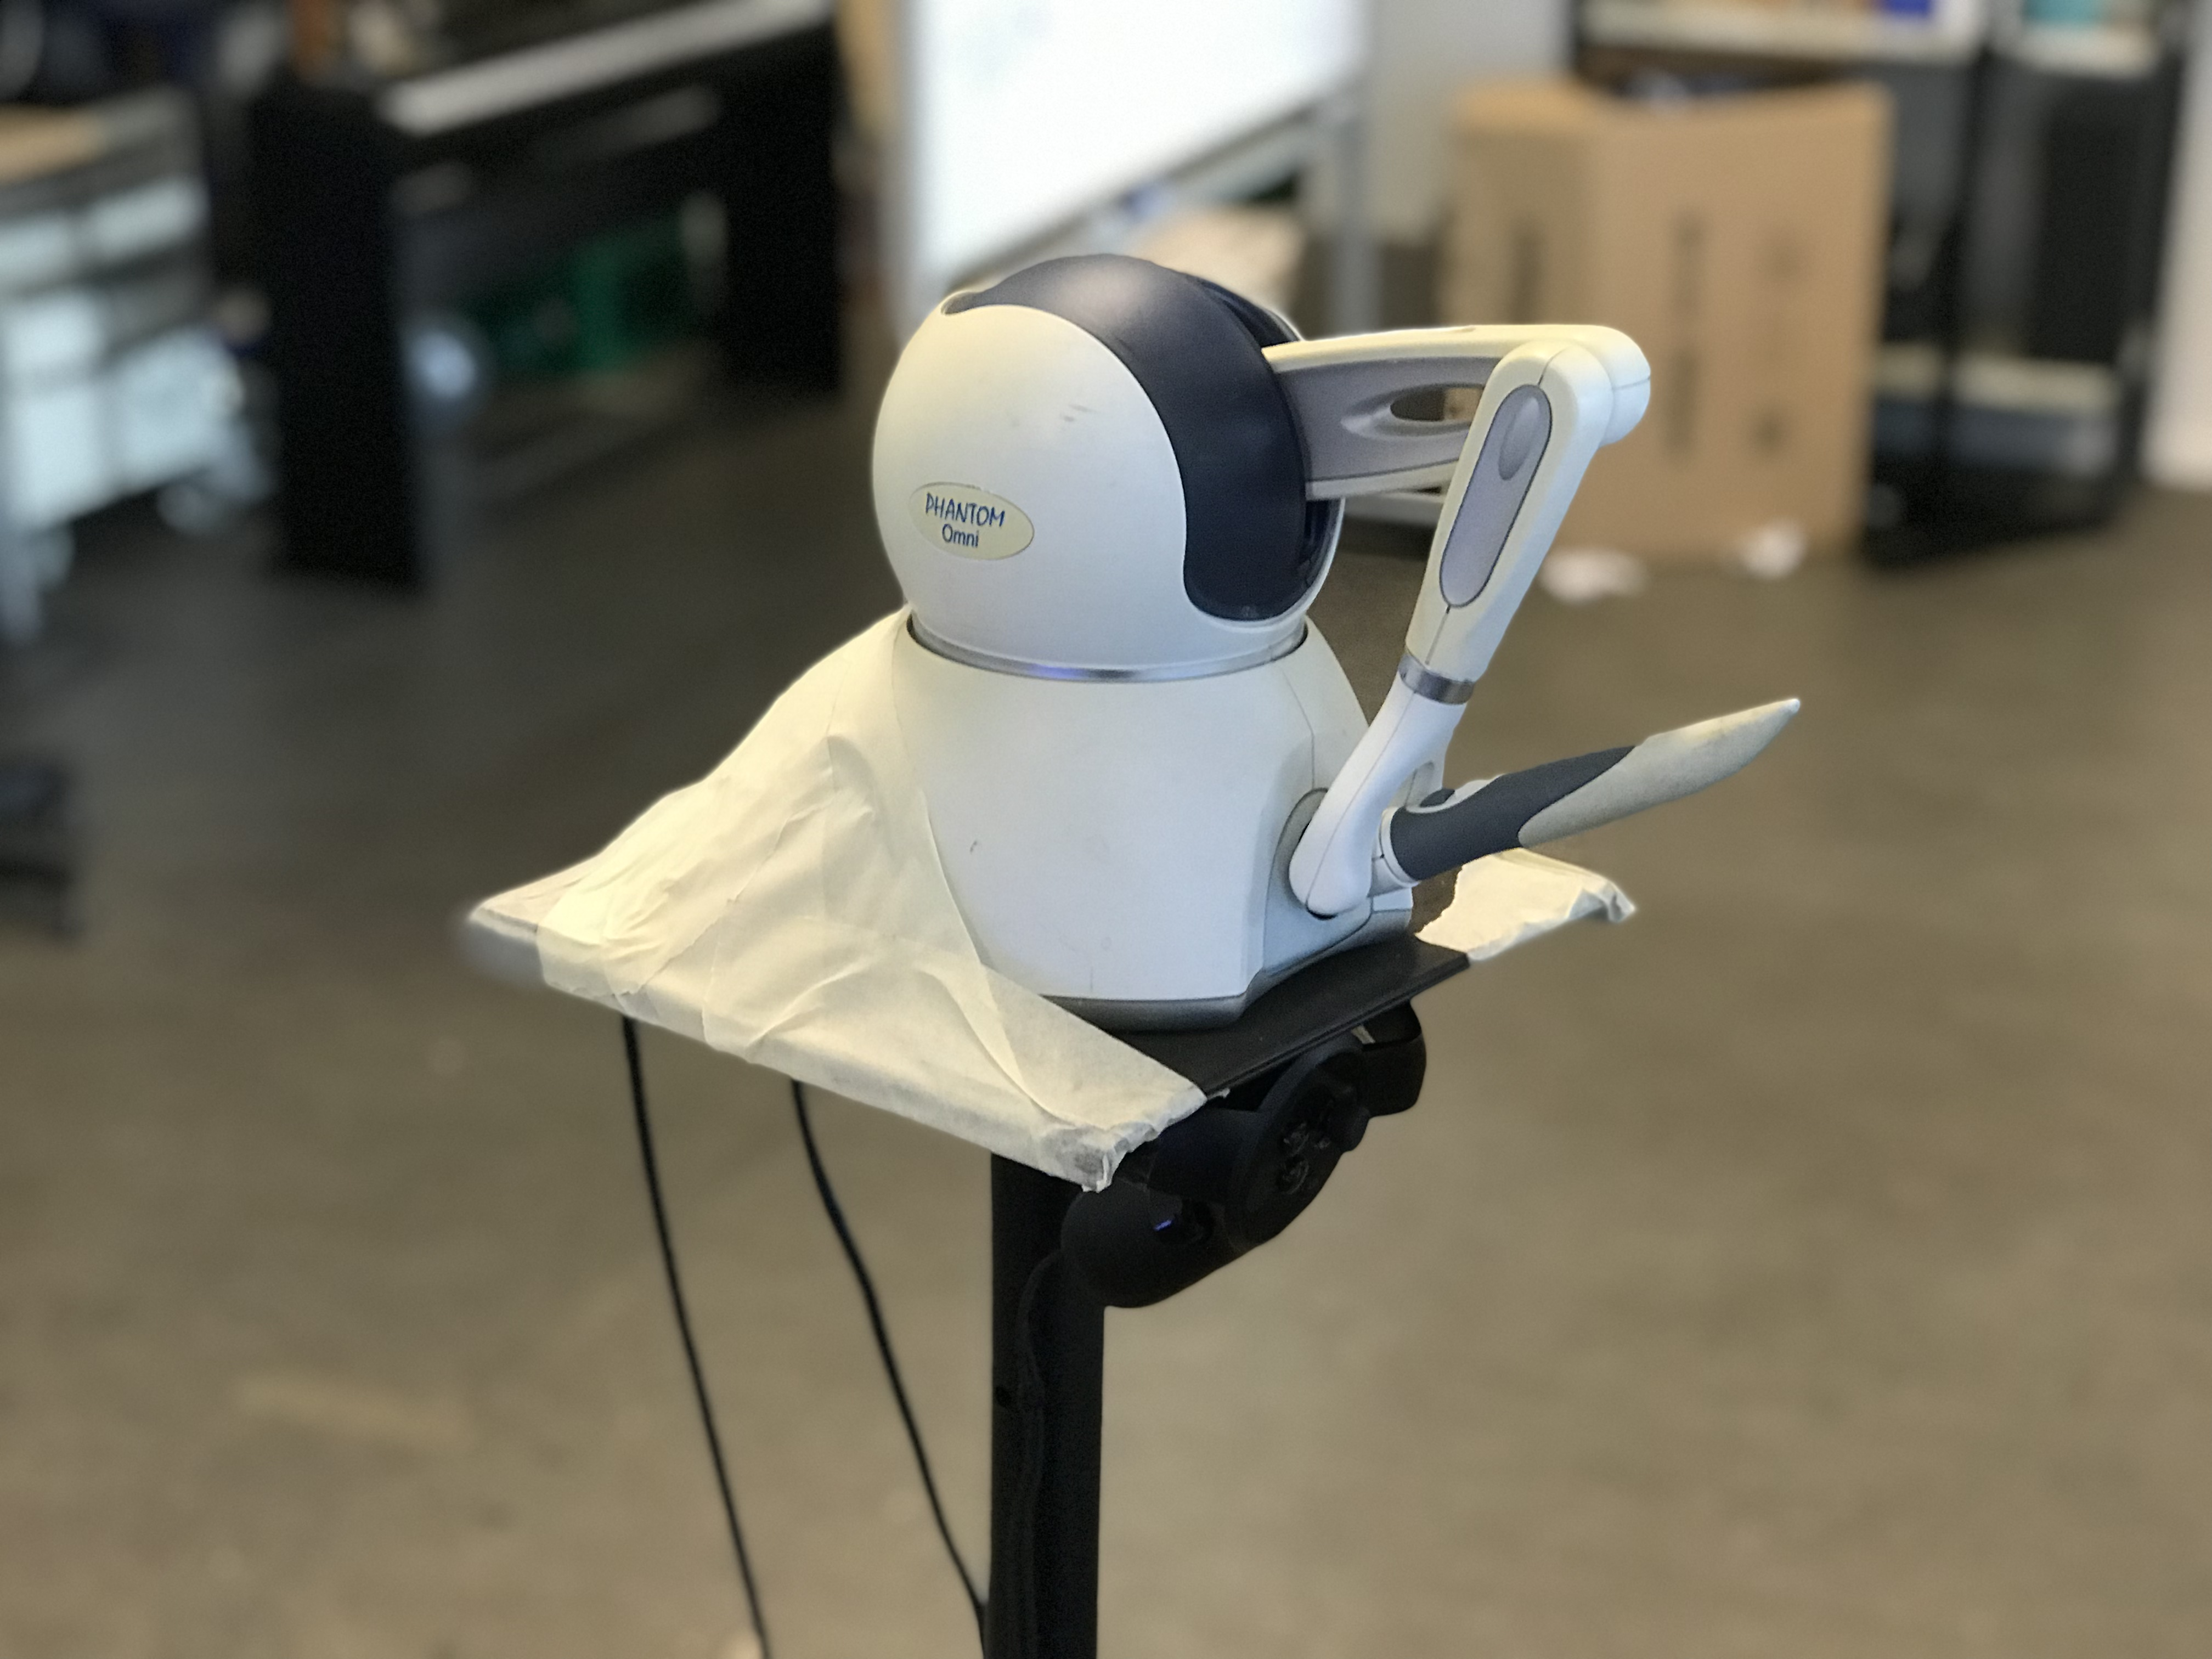
\includegraphics[width=1.0\columnwidth]{SMC 2020 paper template LaTeX/figures/omni.jpg}
% \centering
%   \caption{Diagram showing the system layout of the application. The user interacts with the system using the Omni -- which in turn provides haptic feedback -- and the Oculus Touch controller. These trigger the physical model of the tromba marina. Auditory feedback then comes from speakers and visual feedback from the Oculus Rift headset. A detailed explanation can be found in Section \ref{subsec:physicalSetup}. \label{fig:systemLayout}}
% \end{figure}

\begin{figure}[ht]\includegraphics[width=1.0\columnwidth]{SMC 2020 paper template LaTeX/figures/Cumhur.jpg}
\centering
  \caption{User interacting with the physical setup. The Omni is mounted on a \texttildelow125cm stand together with the right Oculus Touch controller used for location and tilting information. \label{fig:physicalSetup}}
\end{figure}

A diagram showing the setup of the system can be found in Figure \ref{fig:systemLayout}. The user controls the application using the Omni and the left Oculus Touch controller which sends data to the computer running the application. The Omni sends haptic data back based on the collision with the `(hidden) collision block' shown in Figure \ref{fig:localGlobal}. This data simultaneously triggers the physical model which sends its output to a pair of speakers. The user wears a HMD that gives visual information about the location of the tromba marina (and medieval scene). The user's position in the VR environment is controlled by the HMD, but this dataflow is not visualised in the diagram. Lastly, the right Oculus Touch controller is attached to the stand the Omni is attached to, and sends position and tilting data to the application.

\begin{figure}[ht]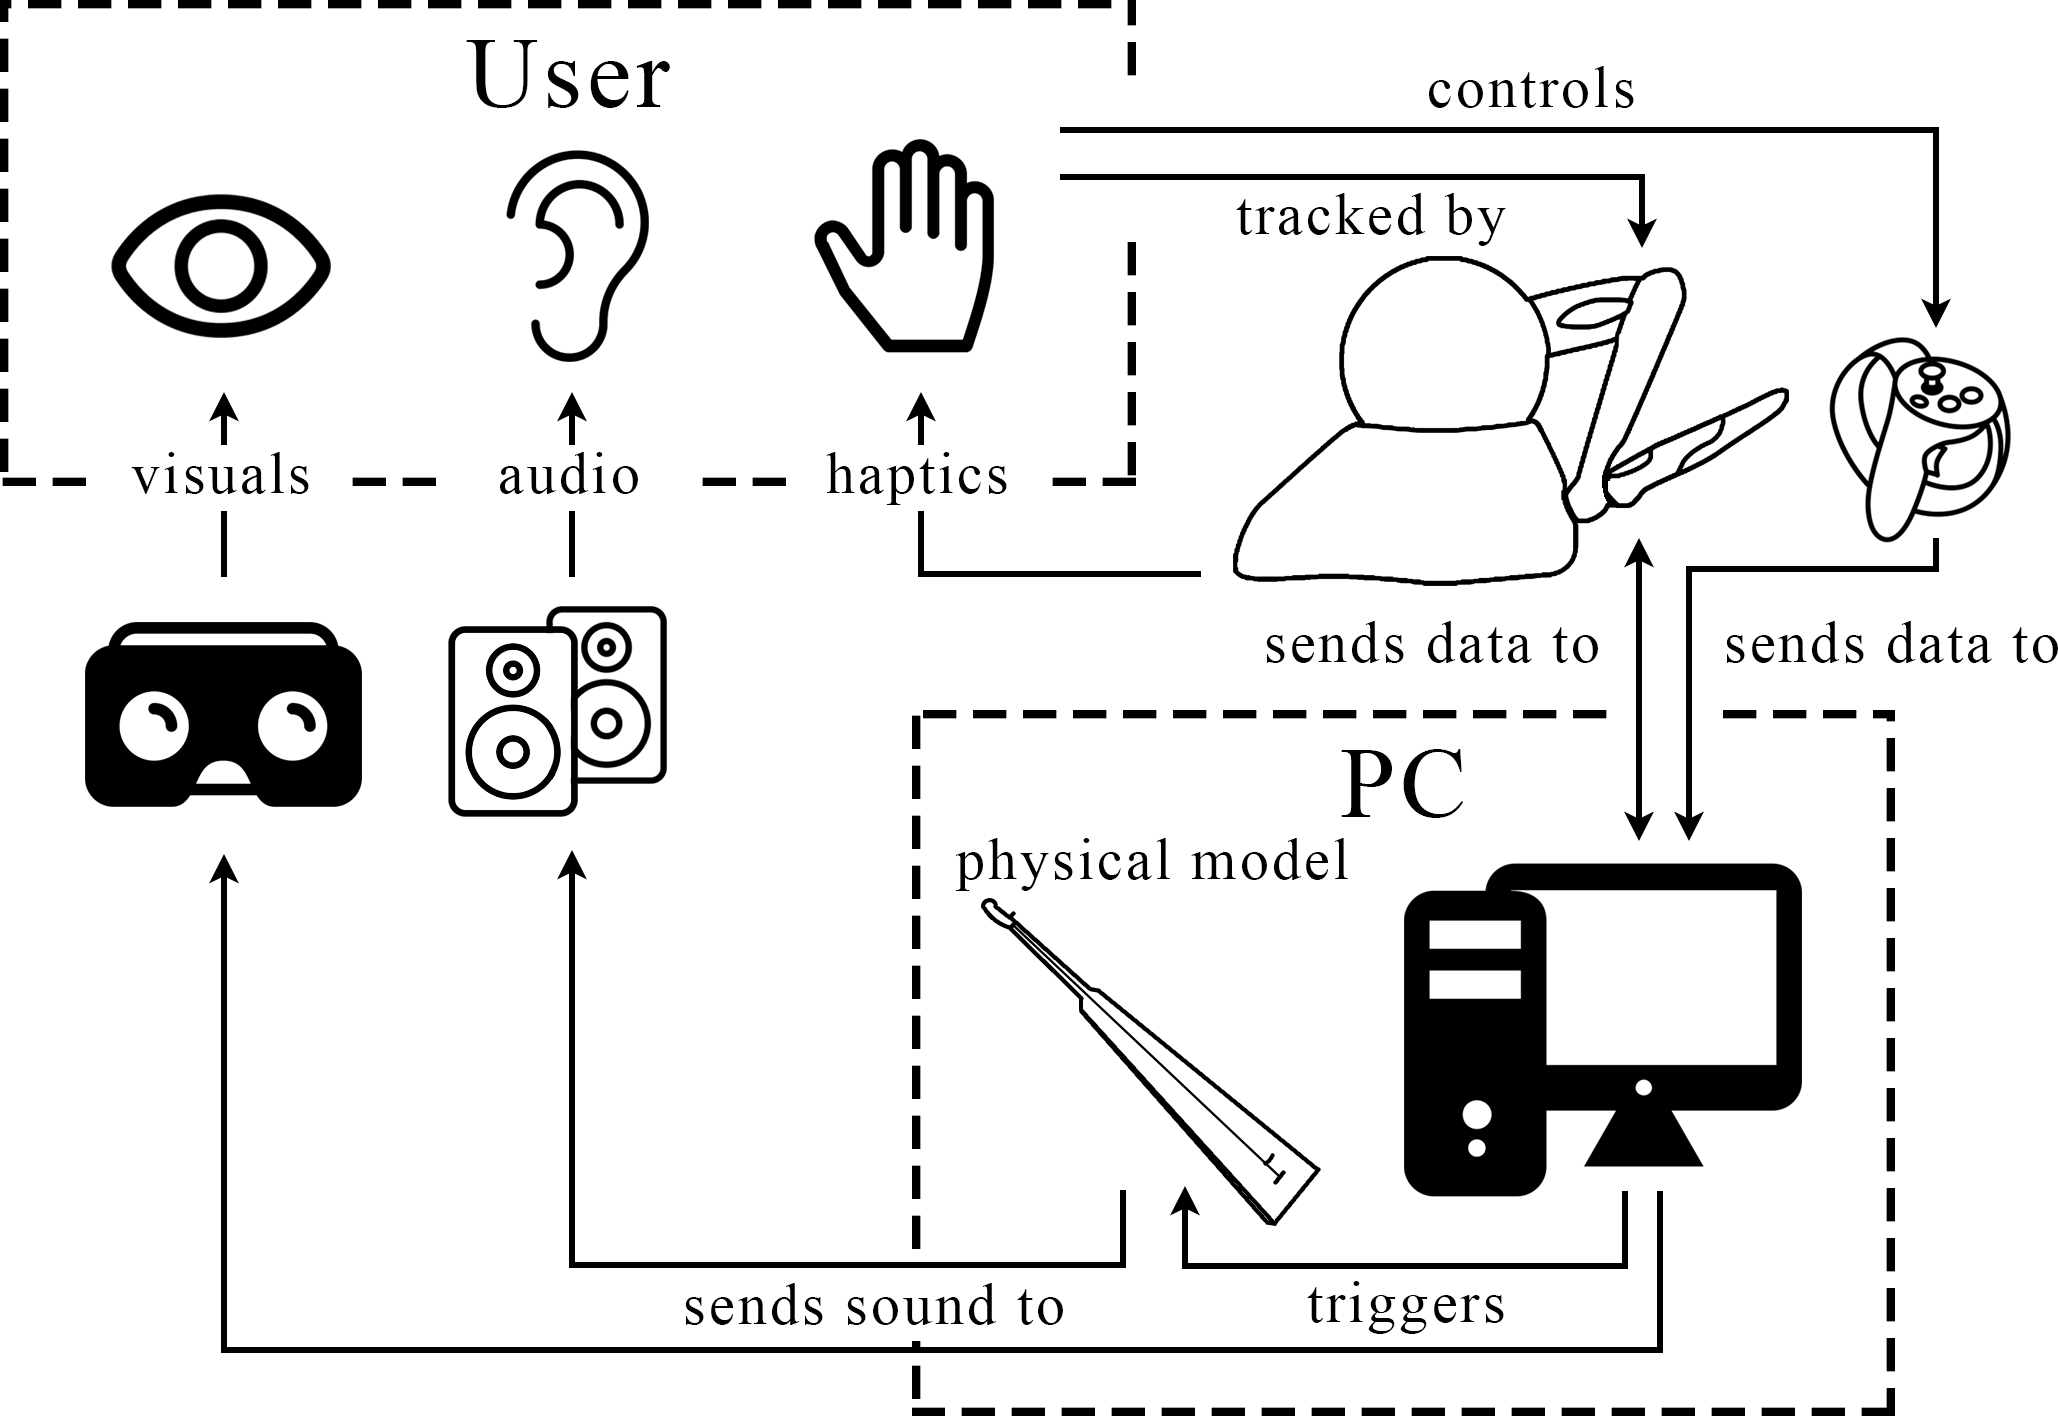
\includegraphics[width=1.0\columnwidth]{SMC 2020 paper template LaTeX/figures/blockdiagram.png}
\centering
  \caption{Diagram showing the system layout of the application. The user interacts with the system using the Omni -- which in turn provides haptic feedback -- and the Oculus Touch controller. These trigger the physical model of the tromba marina. Auditory feedback then comes from speakers and visual feedback from the Oculus Rift headset. A detailed explanation can be found in Section \ref{subsec:physicalSetup}. \label{fig:systemLayout}}
\end{figure}

\section{Evaluation}\label{sec:eval}

The goal of the study was to (1) evaluate the  general experience of bowing in a VR environment using haptic feedback and accurate physical modelling and (2) to evaluate the  playability of a VR monochord instrument. This was done by exploring the quality of the software, the acoustic model, the interface and the mapping, as proposed by \cite{Barbosa2015} and implemented previously in a similar study \cite{Young2003}. To meet this aim, an investigative study was performed through which feedback on the virtual instrument was collected. In order to ensure a high level of validity and reliability, a triangulation of methods has been used: think aloud protocol \cite{Someren1994} throughout the interaction, observation and post-study self report through a modified Usability Metric for User Experience survey \cite{Finstad2010}. The study concluded with an semi-structured interview based on the observed actions, noted comments and questions loosely revolving around \textit{goals, operators, methods and selection} method \cite{Card1983}.

\subsection{Participants}

A total of 14 people (12 male, 2 female), 23-48 years old (M=29.5, SD=7.65)  participated in the study. All participants were students or staff at Aalborg University Copenhagen. The selection of participants was based on the single criterion that one had to have experience playing a musical instrument. Over 70\% of the participants have been playing an instrument for more than 5 years, guitar being the most common occurrence (25\%). There was only one participant experienced in playing bowed instruments (violin). The same participant mentioned playing the tromba marina briefly before, but the majority of the other participants had never heard (of) it. All but one participant have had tried VR experiences before joining the study. 

\subsection{Procedure and Task}

The experiment started with the participant reading an introduction about the experiment and completing a questionnaire covering several demographic questions (age, gender, musical experience, familiarity with the tromba marina and VR experience). They were then introduced to the setup and task, and controls were explained. The participants were informed that the study is exploring the experience of bowing in a VR environment. It was emphasised that the most important part of the experiment was for the participant to talk aloud with the phrase: ``anything positive, negative, basically anything that comes to mind, please speak out loud". Furthermore, the user was instructed to bow above the damping finger (visualised as a white sphere) at all times, as this is also the interaction with the real instrument. 

The interaction part was divided into two phases. Firstly, the participants were asked to freely explore the instrument on their own. Then, when they felt they are ready to move on, an audio recording made by the authors using the application was played, showcasing the system's capabilities, aiming to inspire the second phase of free exploration. It was stressed that the participants did not have to recreate what they heard, but to merely use it as inspiration. The experiment concluded with participants completing a questionnaire covering usability and playability of the system. Finally, a semi-structured interview was held which lasted 5 minutes on average. 

Throughout the interaction phase, the participants' actions were observed and noted by the authors, and their comments written down. Most participants were re-encouraged to think aloud during their exploration. The full experiment lasted \texttildelow30 minutes for all participants.
\subsection{Measurements}

Because the  goal of the study was to investigate the overall experience of bowing in VR, as well as evaluate the playability of the instrument,  self-reporting measurements were used in combination with the observations, interview and \textit{think aloud} notations. Specifically, after exposed to the instrument, the participants were asked to fill out a questionnaire containing 20 items related to the experience of interacting with the VRMI. The items can be broadly segmented into four categories: overall experience, haptic feedback, auditory feedback and visual feedback. Table \ref{tab:questions} presents the questions.

\begin{table}[h]
\centering
  \small
    \begin{tabular}{p{0.95\columnwidth}}
    \textbf{Questionnaire items:} \\
    \hline
    \\[-0.1in]
    \textit{Overall experience:} \\
    (1) It was easy to understand how to play the instrument.\\
    (2) I felt the instrument was hard to play.\\
    (3) I felt the instrument was expressive.\\
    (4) The instrument's capabilities did not match my expectations.\\
    (5) I felt I could easily achieve my goals.\\
    (6) I made many errors playing the instrument.\\
    (7) I am satisfied with the instrument.\\
    (8) I felt the instrument was boring.\\
    (9) Interacting with the instrument was frustrating.\\
    \hline
    \\[-0.1in]
    \textit{Haptic feedback:}  \\
    (10) I felt the haptic feedback was realistic.\\
    (11) I felt the haptic feedback was too strong.\\
    (12) I felt the haptic feedback was natural.\\
    \hline
    \\[-0.1in]
    \textit{Auditory feedback:}\\
    (13) I felt I was in control of the sound.\\
    (14) I felt the audio was matching my actions.\\
    (15) I felt the sound was matching the haptic feedback.\\
    (16) I felt the sound was matching the visuals.\\ 
    (17) I felt the sound was static.\\ 
    \hline
    \\[-0.1in]
    \textit{Visual feedback:}\\
    (18) I felt the visual feedback was helping me play.\\
    (19) I felt the visuals were confusing.\\
    (20) I felt the visuals were matching my actions.\\
    
    \hline
    \end{tabular}%
      \caption{The questionnaire items and corresponding anchors of the 5 point (1-5) rating scales (Strongly disagree -- Strongly agree).}
  \label{tab:questions}
\end{table}
%
\section{Results}\label{sec:results}
This section presents the results obtained from the self-reported measure regarding the participants' experience as well as the qualitative findings from interview, observations and think aloud.

\subsection{Quantitative Data}
The data obtained for the questionnaire items was treated as ordinal and analysed in terms of central tendency (medians and mode), interquartile ranges, minimum and maximum ratings. Figure \ref{fig:boxplots} visualises the collected data. The mode was considered only when different from the median, specifically question 8, 13 and 14. It is worth noting that most of the items show a skewed normal distribution.

Question 1-9 paint a picture of how the instrument was perceived by the users. Questions 1, 2, 4, 5, 6 and 9 cover the perceived difficulty of using the system as a musical instrument. The answers to these questions show that even though participants generally found the instrument easy to understand, they had difficulty playing it and reaching their goals.
Questions 3, 7 and 8 cover their general opinion about the instrument. Participants generally felt satisfied and not bored with the instrument.
Questions 10-12 cover exclusively the impressions about haptic feedback. It can be seen that most participants found the haptic feedback to be realistic and generally natural and the force to be not too strong.
The questions 13-17 approach the auditory aspect of the instrument, focusing on its perceived characteristics. As can be seen from questions 13, 14 and 17, the participants felt a high level of command over the sound, and were satisfied with mapping between the haptic and auditory feedback. The same thing can be said about the visual mapping, as indicated by question 16. 
Items 18-20 investigate the perceived visual quality. It can be seen that the visuals helped the participants play and were implemented well, i.e., not confusing and matching their actions.

\begin{figure*}[!t]
    \centering
    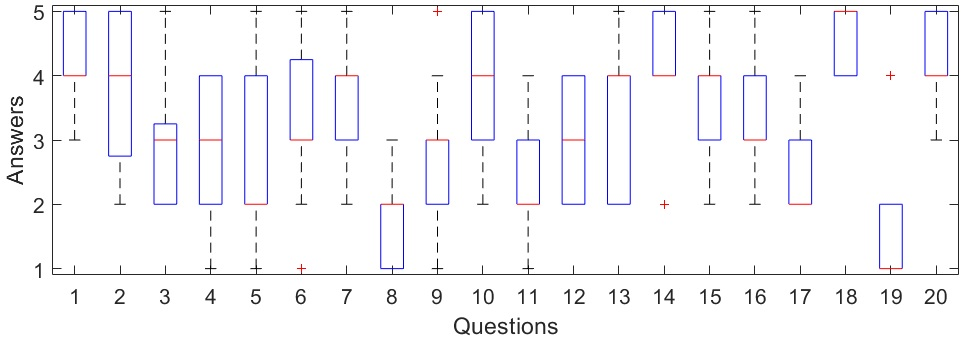
\includegraphics[width=1.0\textwidth]{SMC 2020 paper template LaTeX/figures/Boxplots.jpg}
    \caption{Boxplots visualizing the results related to the 20 questionnaire items in terms of medians, interquartile ranges, minimum and maximum ratings, and outliers. The y-axis maps "Strongly disagree -- Strongly agree" to a 1 -- 5 interval.}
    \label{fig:boxplots}
\end{figure*}

\subsection{Qualitative Data}
In order to present an accurate representation of the findings, this section will be split into two categories: actions -- covering the observed activities during the interaction phase, and oral feedback -- presenting the findings from the think aloud protocol and interviews.

\subsubsection{Observed Actions}
Since there were no tasks given to the participants, all actions were noted and analysed. That said, most users performed similar actions in their interaction phase. All participants experimented with bowing at different heights, but only a few of them tried to explore bowing heights for all discrete pitches. Most of them were satisfied with trying different heights on whatever pitch they found themselves at that time. In a similar fashion, all participants experimented with playing different pitches, both using the discrete buttons as well as the joystick. It is worth mentioning that many users tried to investigate the limits of the pitches they could play. Higher pitches usually resulted in little or no sound which was commented on by most. This behaviour is true to a real tromba marina, where higher harmonics are harder to excite that lower ones. The majority tried to perform some form of glissando, as well as bowing with different velocities, usually commenting on the findings. Due to the non-intrusive nature of observation, it was impossible to notice the pressure applied with the bow, but some participants explicitly mentioned that they tried to experiment with different forces. This was especially true in the second phase of interaction, when they experimented with a higher dynamic range of sounds. Another common occurrence was the attempt to play some sort of melody or riff. Simple melodies like \textit{Mary had a little lamb}, or \textit{Twinkle twinkle little star} were attempted, with various degrees of success. One participant tried to play a Mozart segment. The last commonality was found in the attempt to perform a sustained tone, with a constant bowing speed and a back-and-forth motion.

When it comes to seldom or individual actions, a great variance in experimentation was observed. Participants tried to hit the string with the bow, rotate the bow upwards to the point of it being parallel to the string, move the bow in an up-down (y-axis) motion, bow on the damping finger indicator and underneath it or play some form of vibrato or staccato. No one tried to tilt the stand supporting the Omni.

\subsubsection{Oral Feedback}

Generally the overall impression of the instrument was positive, described with words like: \textit{cool, fun, interesting, weird}, as well as \textit{hard} or \textit{difficult to play}. One participant's answer encapsulates this very well by saying: ``I got to express my ideas, but not perfect them". 

Just as described in the previous section, there was a general consensus on several reported characteristics. All participants that attempted to play the highest harmonic said it is hard to play, and that it felt frustrating. At the other end, several participants expressed their preference towards lower pitches, where some said that they prefer the sound produced when bowing under the damping finger (basically playing the lower-pitched open string). Besides that, many reported that is was hard to maintain a sustained tone, regardless of the pitch. Another sound-related report was the inability to re-create the buzzing sound heard in the recording; one of the participants familiar with the tromba marina's mechanism even mentioned specifically that he ``couldn't get the bridge to rattle". When it comes to the pitch selection interface, the reports are very polarised between the joystick and the buttons. On one hand some describe the buttons as being more, \textit{fun, musical, melodic, useful} or \textit{easier}, while describing the joystick as \textit{useless, unrealistic, too hard} or \textit{meaningless}. On the other hand some participants clearly preferred the joystick describing it as \textit{natural, intuitive, interesting, expressive} or \textit{humane}, but everyone mentioned that the sensitivity of the joystick is too high, making it hard to land on the desired pitches. Due to the incremental nature of the damping fingers' position, it was impossible to skip over notes, a fact that was mentioned in different forms by several participants. Some noted that the control of the damping finger (`Y' for up the string and `X' for down) should have been inverted. Furthermore, some would have liked a more physical interaction for the damping finger, such as moving the controller up and down rather than using buttons.

When it comes to the haptic feedback the majority was satisfied with it, mentioning that ``it feels nice", ``it feels good", ``is great", ``impressive - it felt natural", or ``it feels real", while one participant found it to be ``wild and a bit too powerful". A special case related to the haptic feedback was the bounce obtained by hitting the virtual string with the bow. Most subjects found it pleasing and were intrigued by it's realistic feel, but the violin player repeatedly mention that it is "unrealistic and way to powerful". One participant explicitly mentioned that the haptic feedback matches the auditory one, and his expectations.

Several participants noticed that the bow could rotate along its axis and asked whether it made a sonic difference or not, to which they were answered negatively. Besides that, there were very few comments regarding the visual aspect of the system, but most of these were positive. One participant mentioned that sometimes there's a gap between the string and the bow, and that it would be nice to observe one's hands.  No one mentioned anything related to the visual indication or the damping finger seen in Figure \ref{fig:vrView}.

The overall interaction was described offering a high degree of freedom on the bowing hand, but the pitch selecting hand was either not mentioned, or described as \textit{disconnected} several times. Some agreed that the instrument is hard to play, mentioning that it is \textit{frustrating}. However, most people estimated that they can perform better after practising more.

% \begin{figure}[ht]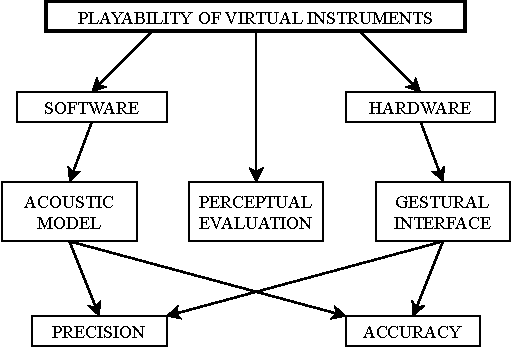
\includegraphics[width=1.0\columnwidth]{SMC 2020 paper template LaTeX/figures/PlayabilityChart.pdf}
% \centering
%   \caption{Playability chart of a virtual musical instrument \cite{Young2003}. \label{fig:oculusController}}
% \end{figure}

\section{Discussion}\label{sec:discussion}

\ifx
%############################
To cover in discussion chapter
#1. think aloud protocol might be bad 
#2. Example sound - some tried to do replicate but they couldn't - might have influenced the goal question
#3. Bounciness was regarded as really cool and realistic, even though it's more of a byproduct
#4. Bow length and passing through the string - Silvinging
#6. Miss alignment between bow initial position and haptic omni pen - Haptic omni has a gained/exaggerated motion mapping
#7. highest pitch it's hard to excite
#8. joystick is to sensitive, some hate it, some love it
#9. pitch range, and playing below the string
10. no one use the tilting?! p.s. we forgot to mention that we used Peter to help us design. 
11. talk about why the left hand is static

%############################
\fi

%Recalling our goal (at the beginning of Section \ref{sec:eval}) 
In this section, both the evaluation itself and the results from Section \ref{sec:results} will be discussed.

\subsection{Procedure}
It is acknowledged that the cognitive load of speech and playing an instrument are overlapping \cite{Stowell2009}, therefore the \textit{think aloud protocol} might have not generated in the most abundant data possible. Most participants alternated between playing and speaking. This resulted in occasionally long breaks in either activities, and required participants to be encouraged to think aloud. Retrospectively, a structured activity schedule allocating time for playing and feedback could have been more productive. Similarly, using self report through Likert scales require large sample sizes to achieve a high level of accuracy\cite{Stowell2009}. Therefore the interpretation of results rooted into the qualitative data, and then validated using the quantitative data. 

Furthermore, the audio did not fully match the sounds that were possible to create with the application. As the recording was quite distorted, the volume of the audio plugin was turned down during the test, but the recording was not remade. This will be elaborated on below.

\subsection{User Feedback}
The generally positive oral feedback about the overall experience is backed up by the quantitative data which showed that participants were satisfied and not bored with the instrument. They attempted to perform fundamental tasks as producing a sustained tone or playing simple melodies with various degrees of success, and when exposed to the example recording, some tried to recreate the sounds heard from the audio clip. Several participants mentioned that it was difficult to achieve this particular goal, a problem that finds its explanation in the difference in volume between the recording and the experiment scenario as mentioned above. This would be a point of improvement for future testing, as it could have impacted the answers for question 5 -- the lowest scoring question regarding the overall experience. Another reason for this question's answers could be linked to the inability to play the higher notes, or the limited pitch range, as presented in Section \ref{sec:results}, but these characteristics are inherited from the physical characteristics of the real instrument, so could be expected.

Interestingly, many participants believed that it was easy to understand how to play the instrument, but that they could become better after some more practice. %This can also be seen from the participants' answers to the questions covering perceived difficulty. 
This indicates that the setup has a low ``entry-level", with an envisioned high virtuosity ceiling. This is believed something desirable when creating computer based instruments \cite{Wessel2002}. Even though the implementation was inspired by a real instrument with a possibly different learning curve, as mentioned, it was not our goal to recreate it.  

The haptic feedback was considered positive and generally having an appropriate level of resistance to movements. The answers to questions 10 (realistic haptic feedback) and 12 (natural haptic feedback) correlate positively and question 15 (sound matching the haptic feedback) was also answered positively, giving a strong indication that the participants considered the haptic feedback real and according to their expectations.  It can be understood that the realism of the haptic feedback is estimated considering the multisensory experience and this result reassures that bowing in VR with our setup is possible.

Furthermore, many participants noticed that they could `bounce' the bow onto the string. Even though this behaviour was a byproduct of the implementation, participants generally liked this interaction and found it to be realistic and exciting.  

Many users noted that the full range of the bow could not be used. As mentioned in Section \ref{subsec:physicalSetup}, the virtual tromba marina was aligned with the physical position of the Omni and as the bow is held at one end, about half of the range could not be used for bowing. This was a common reported issue, and it could have impacted the answers for question 4, 5, and 9. The reason for aligning the physical setup with the virtual tromba marina was the tilting interaction, so that if people wanted to interact with the entire instrument, they would be able to grab the physical setup. As none of the participants used this, we could get rid of the aforementioned alignment to be able to account for the entire range of the bow. %This was done in an attempt to compensate for the inconsistency between the movements of the bow in the real world, and the virtual world. This inconsistency was due to the fact that the Phantom Omni's Unity3D plugin applies an unknown gain coefficient to translation motions.  

The polarisation of the participants' opinion on the pitch control -- joystick versus buttons -- was backed up by the answers individuals gave on question 9 (interaction was frustrating). It could be argued that users preferring the joystick over the buttons had a harder time interacting with the instrument than the people preferring the buttons. As mentioned, all participants who mentioned the joystick interaction said it was too fast, explaining the above.

\section{Conclusions} \label{sec:conclusion}
This paper presents a virtual reality implementation of the tromba marina and its evaluation. Our goal was to evaluate the general experience of bowing in VR and to evaluate the playability of our implementation. The results show that the implementation was successful with participants finding the haptic feedback realistic and the general experience enjoyable and interesting on one hand, and difficult and frequently frustrating on the other hand. Nevertheless, all sensory modalities we focused on (auditory, haptic and visual) seemed to reinforce each other, inspiring participants to attempt to play melodies with the instrument. This was considered to be an important achievement.
Improvements on our application include the pitch control, which  should either be more physical, i.e., moving the pitch hand physically up and down the virtual string, or simply slower continuous control. Besides that, a more optimal physical setup, allowing the users to utilise the entire bow is desired.
The findings of this paper prove that it is possible to create a satisfactory bowed VRMI using off the shelf hardware and accurate physical modelling. 

\begin{acknowledgments}
We would like to thank all participants for taking the time to evaluate our implementation. We would especially like to thank Peter Williams for his valuable insights on playing the tromba marina, feedback on our application and providing access to his instrument replica. 

This work is supported by NordForsk's Nordic
University Hub Nordic Sound and Music Computing Network
NordicSMC, project number 86892.
\end{acknowledgments} 

%%%%%%%%%%%%%%%%%%%%%%%%%%%%%%%%%%%%%%%%%%%%%%%%%%%%%%%%%%%%%%%%%%%%%%%%%%%%%
%bibliography here
{
\small
\bibliography{smc2020bib}
}
\end{document}
